

\begin{figure}[ht]
\centering
\begin{subfigure}{.33\textwidth}
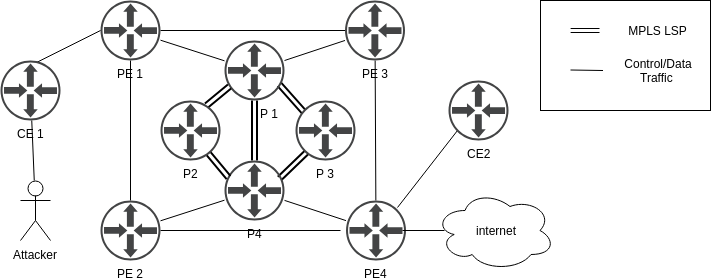
\includegraphics[width=\linewidth]{resource/img/ch_background/sdn_analytics/use_case_figs/mig_step_001.png}
\caption{Current}
\label{fig:current}
\end{subfigure}%
\begin{subfigure}{.33\textwidth}
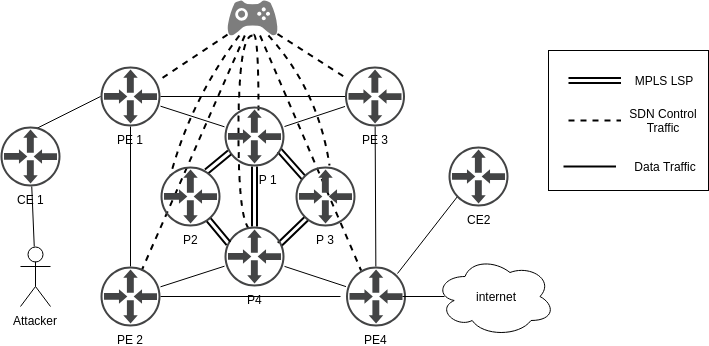
\includegraphics[width=\linewidth]{content/chapters/ch_background/sdn_analytics/2/figs/use_case_figs/mig_step_002.png}
\caption{Transition}
\label{fig:trans}
\end{subfigure}%
\begin{subfigure}{.33\textwidth}
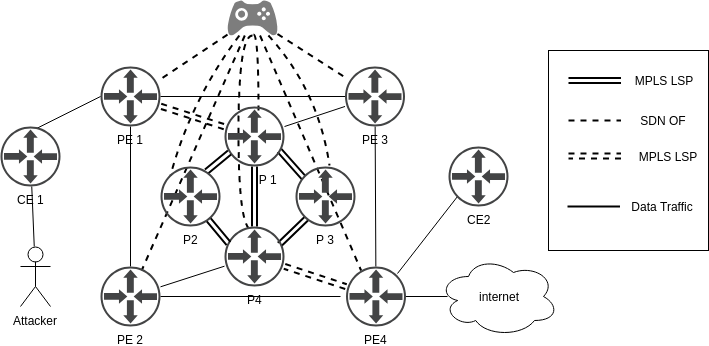
\includegraphics[width=\linewidth]{content/chapters/ch_background/sdn_analytics/2/figs/use_case_figs/mig_step_003.png}
\caption{Future}
\label{fig:future}
\end{subfigure}%
    \caption{Network migration models from current to future}
\end{figure} 


The primary network elements we consider for this analysis are \textit{Customer Edge (CE)} routers, \textit{Provider Edge (PE)} routers, and \textit{Provider Core (P)} routers. \textit{CE} routers attach to \textit{PE} routers and communicate information about the customer network  topology to the provider. \textit{PE} routers exchange routing information with other \textit{PE} routers about the networks they are attached to. \textit{PE} routers also learn from \textit{P} routers what paths are available through the provider network.  Once routing and signalling information is established, the \textit{PE} and \textit{P} routers can forward customer traffic through the provider network. In conventional networks routing and signalling information is exchanged directly between adjacent routers, whereas the controller receives this information in SDN architectures. To determine the correct path through the network, routers and switches are required to parse frame and packet headers to identify the source and destination of incoming traffic. \textit{Multi Protocol Label Switching (MPLS)}\cite{Awduche_Agogbua_1999} is used to reduce the overhead of packet processing and isolate customer traffic by applying labels on incoming packets. Labels speed up routing through core and transit networks by reducing the effort needed to process the header at each hop. We have reduced the scale and scope of the network models to capture some of the key changes in the architectures during migration while reducing overall complexity. These representative models allow us to isolate the impact of specific architecture changes on the system’s security.  %Follow on efforts to leverage existing network mapping, network management, and vulnerability scanning tools will enable automated generation of more accurate and near real time network models. This work could be incorporated into the existing security incident event management (SIEM) system for visibility into the security effects of hardware or software level changes on the network.  

The current network model depicted in Figure \ref{fig:current} captures the existing architecture elements such as distributed routing protocols and hardware and operating system level components. When customer traffic enters the Ingress Router PE1 from the customer edge CE1, access control lists are enforced to drop any packets with a destination address matching the address of the core infrastructure. Traffic flows that are not denied by the ACL are then routed through the MPLS core and forwarded to the appropriate Egress Router. In practice, the number of ACL rules maintained on each Ingress Router could exceed 100,000 entries.  

The transition state network in Figure \ref{fig:trans} retains the same logical connectivity as the current network by leveraging ACLs to restrict customer traffic. This model introduces a global SDN controller along with the supporting infrastructure to facilitate a centrally managed SDN environment. Proprietary switching hardware has been replaced by merchant silicon and the vendor specific applications that control the hardware have been abstracted and moved onto the hypervisor. The result is that, while ACLs can now be centrally managed, the attack surface of the network has increased with the addition of the SDN components.

The final network model in Figure \ref{fig:future} assumes the same underlying infrastructure as the transitional SDN model in \ref{fig:trans} but places the user traffic bound for the internet in an MPLS VPN tunnel\cite{Muthukrishnan_Malis}\cite{Rosen_Rekhter_2006} instead of the default global routing context. This allows us to study the overall effect on security of isolating the customer traffic flows and preventing the core elements from being directly addressable.  

% current
\begin{table}[ht]
\caption{Network Elements}\label{tab:current_elements}
% \resizebox{.6\textwidth}{!}{%
\begin{tabular}{@{}llll@{}}
\toprule
Device               & Version              & Function        &  \\
 \midrule
Cisco 12000 series   & IOS 12.0(32)S11v     & Provider Edge     &  \\
Cisco ASR9000 series & IOS XR Version 4.3.1 & Provider Edge     &  \\
Cisco CRS1           & IOS XR Version 4.3.3 & Provider Edge     &  \\
Juniper T-series     & Junos 12.3R3-S4.10   & Provider Edge     &  \\
Cisco CRS1           & IOS XR Version 4.2.4 & Core            &  \\
Juniper M320         & Junos 13.2R2-S5.2    & Route Reflector &  \\
\midrule
Merchant Silicon switches, routers, OLTs & Open Network Linux & Fabric &  \\
SDN Controller (local) & Juniper Contrail & SDN &  \\
SDN Controller (global) & ECOMP & SDN &  \\
SDN Controller OS & Ubuntu 14.04 & Application Host &  \\
Network Function Virtualization Host & RHEV 2.2/ KVM 83 & Hypervisor (PE/P/RR/TE) &  \\
Merchant Silicon switches, routers, OLTs & Open Network Linux & Fabric &  \\ 
\bottomrule
\end{tabular}
% }
\end{table}


% % sdn and mpls
% \begin{table}[ht]
% \caption{Transition and Final Network Elements}
% \label{tab:sdn_elements}
% \resizebox{\textwidth}{!}{%
% \begin{tabular}{@{}llll@{}}
% \toprule
% Device & Version & Function &  \\ \midrule
% Merchant Silicon switches, routers, OLTs & Open Network Linux & Fabric &  \\
% SDN Controller (local) & Juniper Contrail & SDN &  \\
% SDN Controller (global) & ECOMP & SDN &  \\
% SDN Controller OS & Ubuntu 14.04 & Application Host &  \\
% Network Function Virtualization Host & RHEV 2.2/ KVM 83 & Hypervisor (PE/P/RR/TE) &  \\
% Merchant Silicon switches, routers, OLTs & Open Network Linux & Fabric &  \\ \bottomrule
% \end{tabular}%
% }
% \end{table}



Some information describing the components of the three architectures is given in Table \ref{tab:current_elements}, while the ports, protocols, and services listing in Table \ref{tab:pps} provides details on current and target state network services. How services are accessed across boundaries, what vulnerabilities are present, and how data flow shifts when moving from decentralized to centralized control are the key elements in this analysis. These details are translated into the MulVal input model described in Section \ref{ch:automation}. %While this list may not be exhaustive, it serves as a starting point to identify areas of the network that are visible to attackers. 

% PPS
\begin{table}[ht]
\caption{Ports, Protocols, and Services}
% \resizebox{.6\textwidth}{!}{%
\begin{tabular}{lllll}
\toprule
Protocol & Port & Service & Boundary &  \\ 
\midrule
IGP & - & OSPF & P &  \\
TCP & 179 & BGP & PE$\leftrightarrow{}$PE,$\quad$ PE$\leftrightarrow{}$CE &  \\
TCP/UDP & 363,1698,1699 & RSVP & P &  \\
PIM & - & - & P &  \\
Telnet & - & Telnet &  &  \\
TCP & 22 & SSH &  &  \\
UDP & 161,162 & SNMP &  &  \\
UDP & 123 & NTP &  &  \\ 
\midrule
IGP & - & OSPF & P $\leftrightarrow{}$SDN local &  \\
TCP/UDP & 646 & LDP & P $\leftrightarrow{}$ SDN local &  \\
TCP & 179 & BGP & PE$\leftrightarrow{}$CE and P/PE$\leftrightarrow{}$SDN local \\
TCP/UDP & 363,1698,1699 & RSVP & P $\leftrightarrow{}$ SDN local &  \\
PIM & - & - & P$\leftrightarrow{}$ SDN local &  \\
Telnet & - & Telnet &  &  \\
TCP & 22 & SSH &  &  \\
UDP & 161,162 & SNMP &  &  \\
SAA/TWAMP & - & - &  &  \\
UDP & 123 & NTP &  &  \\
TCP & 6633 & OpenFlow & SDN Global $\leftrightarrow{}$ SDN local &  \\
\bottomrule
\end{tabular}%
% }
\label{tab:pps}
\end{table}